\documentclass[sans serif,9pt,xcolor=dvipsnames]{beamer}%tipo de documento

\usetheme{Copenhagen}% tema a utilizar
%\useoutertheme{infolines}
%\usecolortheme[RGB={50,93,16}]{structure}
\usecolortheme[RGB={123,16,64}]{structure}
\useinnertheme{rectangles}
%79 168 51
\setbeamercovered{transparent}
%para el difumidado de las transparencias
\beamertemplateshadingbackground{gray!20}{purple!20}
% papaquetes personales
\usepackage[spanish]{babel}%paquete de idioma
%la utilizacion de la instruccion anterior puede llevar a que existan errores en los demás paquetes para ello:
\renewcommand{\contentsname}{Contenido}
\renewcommand{\partname}{Parte}
\renewcommand{\appendixname}{Apéndice}
\renewcommand{\figurename}{Figura}
\renewcommand{\tablename}{Tabla}
\renewcommand{\abstractname}{Resumen}

\usepackage[utf8]{inputenc}% utf8 permite la utilizacion de tildes y Ñ directamente del teclado si la distribucion es utf8. Pero si se tiene otra distribucion, el argumento será latin1
\usepackage{geometry} % para margenes
\usepackage{graphicx} % para colocacion de figuras
\usepackage{color}% para colorear el texto
\usepackage{hyperref}%para hacer referencias a las direcciones de paginas en internet
\usepackage{url}% para escribir una URL
\usepackage{ragged2e}

\begin{document}
\title[\LaTeX]{\textbf{\Huge Programación Literaria Investigación Reproducible y Software Libre}}  
\author[Ing. Milton Labanda, Mg.]{Ing. Milton Labanda, Mg.}
\institute[UIDE Informática]{Carrera de Ingeniería Informática y Multimedia\\ Universidad Internacional del Ecuador}

\setbeamerfont{title}{shape=\itshape,family=\rmfamily}%cambiar tipo de letra
%\setbeamercolor{title}{fg=blue!80!black,bg=green!20!white}%comabiar color de letra y color de cuadro

%marco para el pie en el titulo
\begin{frame}
%
\includegraphics[height=0.2\textheight]{imagenes/escudoUNL.png} 
%\hfill 
\includegraphics[height=0.2\textheight]{imagenes/logoSIS.png}
\hfill {Reunión Nacional de Ramas IEEE RNR2015}
\titlepage
\begin{center}
%
\includegraphics[height=0.2\textheight]{imagenes/licencia.PNG} 
\end{center}

\end{frame}

%marco para el contenido
\AtBeginSection [<+-| alert@+>]{
\begin{frame}{Outline} %<beamer>
\frametitle {Contenido}
\tableofcontents [currentsection]
\end{frame}}

%\logo{
\includegraphics[[width=0.7\paperwidth, height=0.7\paperheight]{imagenes/cis} }
%\setbeamertemplate{background canvas} {
\includegraphics[width=\paperwidth,height=\paperheight]{imagenes/cis}}



\section{Programación Literaria}
\subsection{Historia}
\begin{frame}
\frametitle{Historia}
\begin{block}{Como empieza todo?}
\begin{columns}
\column{.1\textwidth} \hspace{0.7cm}
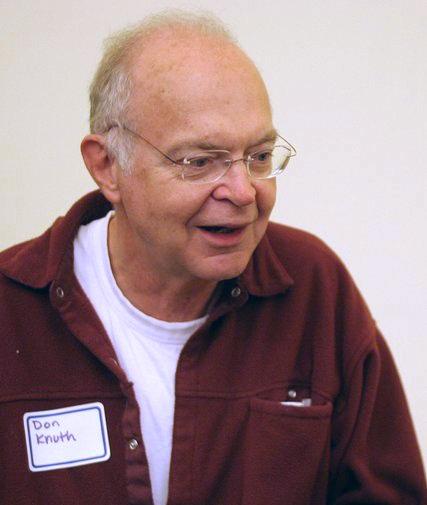
\includegraphics[width=1.8cm]{imagenes/donald.jpg}
\column{.8\textwidth}
\justifying
"I believe that the time is ripe for significantly better documentation of programs, and that we can best achieve this by considering programs to be works of literature. Hence, my title: "Literate Programming" \textbf{\textit{Donald Knuth}}
\end{columns}
\end{block}

\begin{block}{El objetivo}
\begin{columns}
\column{.1\textwidth} \hspace{0.7cm}
%\includegraphics[height=1.5cm]{imagenes/images.png} 
\column{.8\textwidth}
\justifying
Computer programs should be written in a combination of the programming language (the usual source code) and the natural language, which explains the logic of the program. \textbf{\textit{Donald Knuth}}
\end{columns}
\end{block}

\end{frame}

\begin{frame}
\frametitle{Historia}

\begin{block}{WEB}
\begin{columns}
%\column{.1\textwidth} %\hspace{0.7cm}
% % %
\includegraphics[width=1.8cm]{imagenes/latex.png} 
\column{.8\textwidth}
\justifying
Primera herramienta de implementación de lo que se conoció como Programación Literaria. Producía código PACAL compilable y la documentación formateada usando Tex
\end{columns}
\end{block}

\begin{block}{CWEB}
\begin{columns}
%\column{.1\textwidth} %\hspace{0.7cm}
% % %
\includegraphics[width=1.8cm]{imagenes/latex.png} 
\column{.8\textwidth}
\justifying
Descendiente del entorno WEB usa en cambio C como lenguaje de programación pero el mismo Tex para la generación de la documentación
\end{columns}
\end{block}
\end{frame}

\subsection{?`Qué es la Programación Literaria o Estadística?}
\begin{frame}
  \frametitle{?`Qué es la Programación Literaria ?}
\begin{itemize}
\justifying
\item Paradigma cotrario a la programación tradicional: En vez de escribir código que contiene documentación el programador literario escribe documentación que contiene código. 
\bigskip
\item Los Programas literarios pueden ser tejidos (WEAVED) para producir documentos legibles para los humanos y enredados (TANGLED) para producir documentos legibles para las máquinas"

\end{itemize}
\end{frame}

\subsection{Elementos de la Programación Literaria}
\begin{frame}
  \frametitle{Elementos de la Programación Literaria}
\begin{itemize}
\justifying
\item Cada "trozo" de código fuente carga datos y calcula resultados mientras que el código de presentación formatea los resultados (tablas, figuras, imágenes, video, etc.\pause
\bigskip
 \item De los conceptos anotados se desprende que este paradigma requiera: \pause
\begin{enumerate}
\item Un lenguaje de documentación (human readable) \pause
\item Un lenguaje de programación (machine readable) \pause
\end{enumerate}
\end{itemize}
\end{frame}

\subsection{Ejemplos de implementaciones o entornos}
\begin{frame}
  \frametitle{Ejemplos de implementaciones o entornos}
\begin{itemize}
\justifying
\item Sweave = Latex + R
\bigskip
\item  kintr = HTML + R
\bigskip
\item IPython Notebook = HTML + Python
\end{itemize}
\end{frame}


\section{Investigación Reproducible}
\subsection{Por qué y para qué la necesitamos?}
\begin{frame}
\frametitle {Investigación Reproducible}
\justifying
\begin{block}{?`Que persigue?}
\LARGE Hacer los \textbf{datos analíticos} y el \textbf{código} disponibles para que otros puedan reproducir los descubrimientos
\end{block}
\end{frame}


\begin{frame}
\frametitle{?`Por qué necesitamos Investigación Reproducible?}
\begin{block}{... hoy más que nunca}
\begin{itemize}
\justifying
\item Las nuevas tecnologías incrementan las colecciones de datos cada vez más
\item Los datos son más complejos y extremadamente multidimensionales
\item Las bases de datos existentes pueden ser mezcladas dentro de "mega bases de datos"
\item La capacidad de cómputo es altamente incrementable permitiendo análisis mas sofisticados
\item Para cada campo 'X' existe un campo "Computacional 'X'

\end{itemize}
\end{block}
\end{frame}

\subsection{El Análisis de Datos}
\begin{frame}
\frametitle{El Análisis de Datos }
\justifying
\begin{block}{Su estructura}
\begin{itemize}
\item Definir la pregunta
\item Definir el dataset ideal
\item Determinar que datos se pueden acceder
\item Obtener los datos
\item Limpiar los datos
\item Análisis de Datos exploratorio
\item Modelamiento/predicción estadístico
\item Interpretar los resultados
%\item Mejorar los resultados
\item Escribir/sintetizar los resultados
\item Crear código reproducible
\end{itemize}
\end{block}
\end{frame}

\begin{frame}
\frametitle{El flujo tipico de la investigación }
\justifying
\begin{block}{}
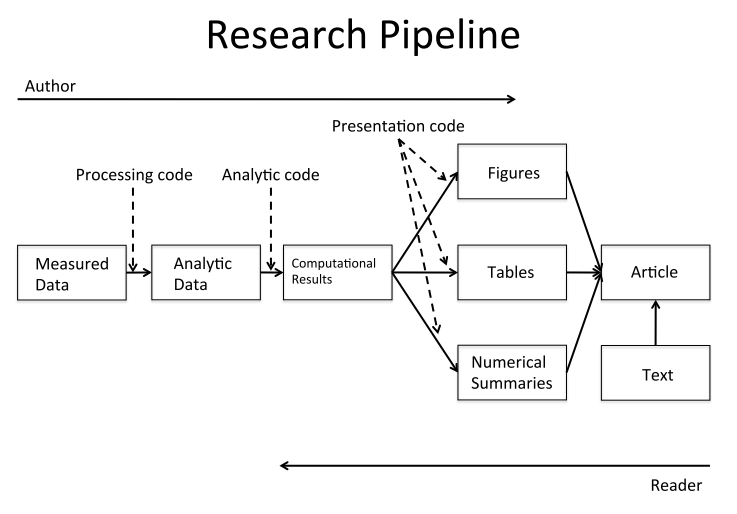
\includegraphics {imagenes/research_flow.png}  
\end{block}
\end{frame}

\begin{frame}
\frametitle{Los actores en el Análisis de Datos}
\justifying
\begin{block}{Autores} 
\begin{itemize}
  \item Desean hacer su investigación reproducible
  \item Quieren herramientas de IR que hagan su vida más facil ("no muy dura")
  \item Relizan considerables esfuerzos para publicar su datos. E: servidor web
  \item Entonces => Con IR colocan solo lo mínimo en la Web así como materiales suplementarios en las revistas o en bases de datos centrales
\end{itemize}
\end{block}
\begin{block}{Lectores} 
\begin{itemize}
  \item Quieren reproducir y posiblemente expandir los descubrimientos de interés
  \item Quieren herramientas de IR para hacer su vida más fácil ("no muy dura")
  \item Deben descargar datos y juntar las piezas: que datos va con qué codigo?
  %\item Pueden no tener los mismos recursos que los autores
  \item Entonces => Descargan los datos y analizan, juntan el software y ejecutan
\end{itemize}
\end{block}
\end{frame}

\subsection{Análisis de Datos + Programación Literaria}
\begin{frame}
\frametitle{Elementos del Análisis de Datos }
\justifying
\begin{block}{}
\begin{itemize}
\item Datos
  \begin{itemize}
  \item Datos crudos (raw)
  \item Datos procesados
  \end{itemize}
\item Figuras
\begin{itemize}
  \item Figuras exploratorias
  \item Figuras finales
\end{itemize}
\item Código
\begin{itemize}
  \item Scripts borrador/no usados
  \item Scripts finales (R, Julia, Python ...)
  \item Scripts Literarios 
\begin{itemize}
    \item Archivos .rmd (R markdown)
    \item Archivos .ipynb (Jupyter/IPython notebooks)
\end{itemize}    
\end{itemize}
\item Texto:
\begin{itemize}
  \item Archivo de ayuda (README)
  \item Texto del análisis/reporte (pdf, html) generado comunmente por  herramientas de programación literaria
 \end{itemize}
\end{itemize}
\end{block}
\end{frame}

\begin{frame}
\frametitle{Estructura mínima de un reporte de Análisis de Datos}
\justifying
\begin{block}{}
\begin{itemize}
\item \Large Titulo
\item \Large Introducción/motivación
\item \Large Metodos (estadísticos)
\item \Large Resultados
\item \Large Conclusiones
\end{itemize}
\end{block}
\end{frame}


\section{Software Libre}
\begin{frame}
\frametitle {Entronos y herramientas popularizados}
\justifying
\begin{block}{IPython Notebook}
\begin{columns}
\column{.1\textwidth} \hspace{0.7cm}

\includegraphics[width=1.8cm]{imagenes/texmaker.png} 
\column{.8\textwidth}
\begin{itemize}
\justifying
\item Creado por Fernando Perez (estudiante español de ingeniería aeronáutica)
\item Es un entorno completo de computación interactiva en entorno web
\item HTML o Markdown + Python o Julia
\item Permite hacer binding hacia otros lenguajes de programación tales como: R, ruby, shell, entre otros.
\item Puede exportar los documentos resultantes hacia: PDF, HTML, Latex o reveal.js 
\item Incluye soporte Unicode, revisión ortográfica, plegado de código y un visor de pdf y modo de visualización continua.
\end{itemize}
\end{columns}
\end{block}
\end{frame}

\begin{frame}
\frametitle {Entronos y herramientas popularizados}
\justifying
\begin{block}{knitr + RStudio}
\begin{columns}
\column{.1\textwidth} \hspace{0.7cm}

\includegraphics[width=1.8cm]{imagenes/texmaker.png} 
\column{.8\textwidth}
\begin{itemize}
\justifying
\item \textbf{knitr} desarrollado por Yihui Xie mientras realizaba su trabajo de graduación
\item Es una librería escrita en R
\item HTML(o LateX o Markdown) + R 
\item Sus caracteristicas están orientadas a mitigar las limitaciones de SWEAVE.
\item Puede exportar a PDF, HTML o Word
\item \textbf{knitr} es integrable con el IDE \textbf{Rstudio}
\end{itemize}
\end{columns}
\end{block}
\end{frame}


\section{Demos}
\begin{frame}
\frametitle {}
\centering \Huge Demos
\end{frame}

%++++++++++++++++++++++++++

\begin{frame}
\frametitle {Editores \LaTeX \hspace{0.1cm}  con Interfaz Gráfica}
\begin{block}{LyX}
\begin{columns}
\column{.1\textwidth} \hspace{0.7cm}

\includegraphics[width=1.8cm]{imagenes/lyx.PNG} 
\column{.8\textwidth}
\begin{itemize}
\justifying
\item Version 2.0.3  marzo del 2012
\item Principal característica es la interfaz gráfica.
\item Enfoque basado en la estructura del documento y no simplemente en su aspecto.
\item Tiene un editor de ecuaciones totalmente integrado para la creación de contenido matemático
\item LyX se publica bajo una licencia Free Software / Open Source, funciona en Linux/Unix, Windows y Mac OS X, y está disponible en varios idiomas.
\item \textbf{Enlace de Descarga:}\textcolor{blue}{\url{http://www.lyx.org/WebEs.Download}}
\end{itemize}
\end{columns}
\end{block}

\end{frame}

\section{\LaTeX en la web}
\begin{frame}
\frametitle {\LaTeX \hspace{0.1cm}  en la web}
\begin{block}{ScripTeX}
%\begin{columns}
%\column{.1\textwidth} \hspace{0.6cm}
\hfill 
\includegraphics[width=1.4cm]{imagenes/scribtex.jpg} 
%\column{.8\textwidth}
\begin{itemize}
\justifying
\item Funcionalidades: almacenar en nuestra cuenta los documentos creados de forma permanente o compartirlos con otros usuarios para trabajar en equipo.
\item Compatible con dispositivos móviles como el iPhone y iPad
\item Opción de trabajo en línea ideal cuando el software habitual falla
\item \textbf{Enlace}\textcolor{blue}{\url{https://www.scribtex.com/}}
\end{itemize}
%\end{columns}
\end{block}
\end{frame}

\begin{frame}
\frametitle {\LaTeX \hspace{0.2cm} en la web}

\begin{block}{Editor Online de Ecuaciones \LaTeX}
\justifying
Este programa permite practicar lo básico del código LaTeX, muestra en tiempo real el aspecto gráfico que tomarán las expresiones algebraicas
Editor de ecuaciones que genera ecuaciones gráficas (gif, png, swf, pdf, emf).\\
\textbf{Enlace: }\textcolor{blue}{\url{http://rinconmatematico.com/latexrender/}}
\end{block}

\end{frame}

\section{Plug-in para tablas desde Calc}
\begin{frame}
\frametitle {Plug-in para tablas desde Calc}
\justifying
LaTeX puede reutilizar los datos existentes en tablas creadas con las hojas de cálculo de OpenOffice, mediante la macro \textcolor{brown}{\textbf{ Calc2latex}}\\

\textbf{Enlace de Descarga: }\textcolor{blue}{\url{http://calc2latex.sourceforge.net/}}
\end{frame}

\section{Creación de Documentos en \LaTeX}
\begin{frame}
\frametitle {Creación de Documentos en \LaTeX}
\begin{center}
\begin{columns}
\column{.2\textwidth} \hspace{1 cm}

\textbf{Tipos de Documentos:}
\begin{enumerate}
\item beamer
\item articulo
\item report
\item letter
\item book
\end{enumerate}
\column{.8\textwidth}
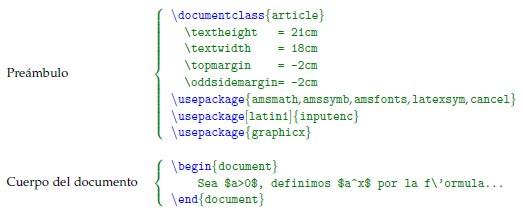
\includegraphics[height=4cm]{imagenes/estDoc.PNG}  
\end{columns}
\end{center}

\end{frame}

\begin{frame}
\frametitle {Creación de Documentos en \LaTeX : Plantillas}
\begin{enumerate}
\item Artículos Científicos
\item Presentaciones
\item Póster
\item Libros
\item Proyectos de Fin de Carrera 
\item Memorias Técnicas
\item Tesis Doctoral
\end{enumerate}
\end{frame}

\section{\LaTeX  en dispositivos portables}
\subsection{VerbTeX LaTex Editor}
\begin{frame}
\frametitle{\LaTeX desde dispositivos móviles}
\begin{block}{VerbTeX LaTex Editor}
\justifying
Es un editor gratuito \LaTeX de colaboración para su dispositivo Android. Te permite crear y gestionar proyectos de \LaTeX directamente en su dispositivo Android y generar un archivo PDF utilizando el servicio de \LaTeX disponible en \textcolor{blue}{\url{http://www.verbosus.com}}  
\end{block}
\begin{center}
\begin{columns}
\column{.2\textwidth} \hspace{0.7cm}

\includegraphics[width=2.5 cm]{imagenes/verbtex.jpg} 
\column{.10\textwidth}
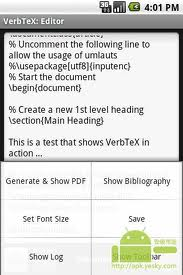
\includegraphics[width=2.5 cm]{imagenes/movilVerbtex.jpg} 
\end{columns}
\end{center}




\end{frame}

\begin{frame}
\frametitle{\LaTeX desde dispositivos móviles}


\begin{block}{ VerbTeX LaTeX Editor: Enlaces de Descarga}
\begin{itemize}
\justifying
\item \textit{Desde el ordenador:}  \textcolor{blue}{\url{http://www.verbosus.com/VerbTeX_v2.1.9.apk}}
\item \textit{Desde el Movil:} 
\begin{itemize}
\justifying
\item Versión Gratuita:\textcolor{brown}{\textbf{VerbTeX LaTeX Editor}}\hfill \textcolor{blue}{\url{Link https://play.google.com/store/apps/details?id=verbosus.verbtex&feature=search_result }}
\item Versión de Pago:\textcolor{brown}{\textbf{VerbTeX Pro LaTeX (Encryption) 1.49 euro }}  \hfill \textcolor{blue}{\url{https://play.google.com/store/apps/details?id=verbosus.verbtexpro&feature=search_result }}
\end{itemize}
\end{itemize}
\end{block}

\end{frame}

\begin{frame}
\frametitle {Versiones de VerbTeX LaTex Editor}
\begin{center}
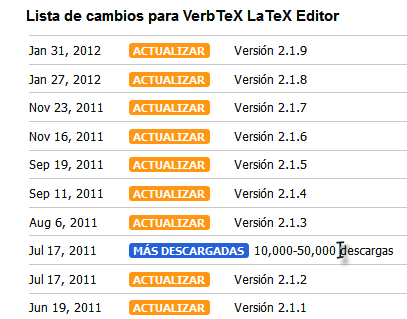
\includegraphics[height=4cm]{imagenes/vMobil.png} 
\end{center}
\justifying
\textbf{Detexify Latex Recognizer}\\
\textit{Enlace al Google Play:}\textcolor{blue}{\url{https://play.google.com/store/apps/details?id=coolcherrytrees.software.detexify&feature=search_result }}
\end{frame}

\subsection{Utilización de USBTeX}
\begin{frame}
\frametitle {Utilización de USBTeX}
\begin{center}

\includegraphics[height=1.5 cm]{imagenes/usbtex.png} 
\end{center}
\begin{block}{Ventajas de USBTEX}
\begin{itemize}
\justifying
\item Es portable(ejecutable en cualquier ordenador Windows)
\item Útil para personas que viajan constantemente
\item Viene empaquetado todas las aplicaciones(Gostscript, Ghostview, un editor y su configuración) necesarios para ejecutar 
\end{itemize}
\end{block}

\begin{block}{Inconvenientes de USBTEX}
\begin{itemize}
\justifying
\item No compila archivos Beamers
\item Solo acepta (*.eps) para imágenes y figuras
\end{itemize}
\end{block}
\end{frame}

\section{Enlaces de Ayuda}
\begin{frame}
\frametitle {Enlaces de Ayuda}
\begin{thebibliography}{10}
\bibitem{  } Alex Borbón A., Walter Mora F.
\newblock{ \LaTeX Composición, Diseño Editorial, Gráficos,
Inkscape, Tikz y Presentaciones Beame} 2012
\newblock 
\url{http://www.tec-digital.itcr.ac.cr/revistamatematica/Libros/LATEX/LaTeX_2011.pdf}

\end{thebibliography}
\end{frame}

\begin{frame}
\frametitle {Créditos}
	\begin{center}
		\textbf{\textit{Expositores}}\\
			Ing. Luis Antonio Chamba Eras\\
			José Fernando Castillo Alba\\
			Gabriela María Narváez Chamba\\
			Jessica Andrea Ponce Calderón\\
			Luis Antonio Soto  Gonzalez\\
\vspace{0.5 cm}
\textbf{\textit{Escritura Científica en \LaTeX }}\\
Grupo de Apoyo para la Escritura Científica\\
  Décimo Módulo\\
  \vspace{0.3 cm}

\includegraphics[height=0.5 cm]{imagenes/escudoUNL.png} \\
\textbf{Universidad Nacional de Loja\\
Carrera de Ingeniería en Sistemas\\
2012
}
	\end{center}
\end{frame}

\end{document}
